\chapter{Langage des expressions booléennes}

\section{Syntaxe}

Ce langage est une extension du langage des expressions arithmétiques qui nous venons de voir.
Nous pouvons également formaliser la syntaxe de notre langage booléen grâce à la notation BNF : \\
$E_B$ ::= true $|$ false $|$ $E_A$ $\le$ $E_A$ $|$ $E_A$ = $E_A$ $|$ not $E_B$ $|$ $E_B$ or $E_B$ $|$ $E_B$ and $E_B$
\vspace{1\baselineskip} \\
De même, nous obtenons le système d'inférence suivant : \\
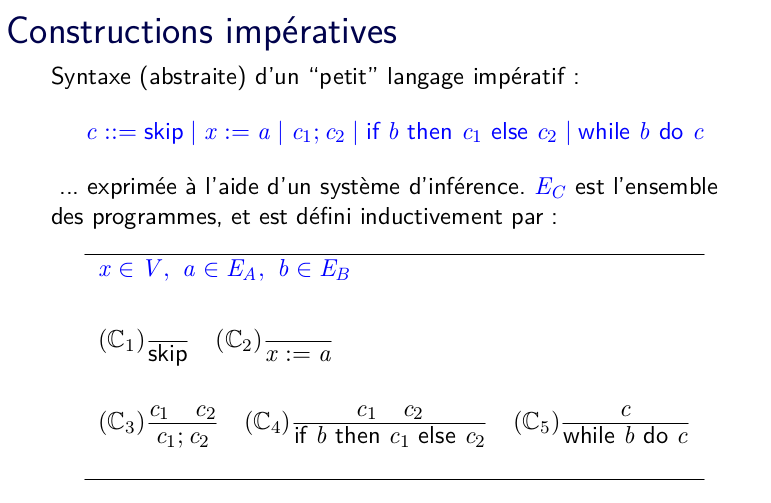
\includegraphics[height=4cm]{\Boolroot/definition_inductive.png}

	\subsection{Traduction en OCaml}
	\lstinputlisting[language=OCaml, linerange={244-249}]{\OCamlroot/OCaml_exemple.ml}

	\subsection{Traduction en K}
	\lstinputlisting[language=K, linerange={41-51}]{\Kroot/K_exemple.k}

\section{Sémantique dénotationnelle}





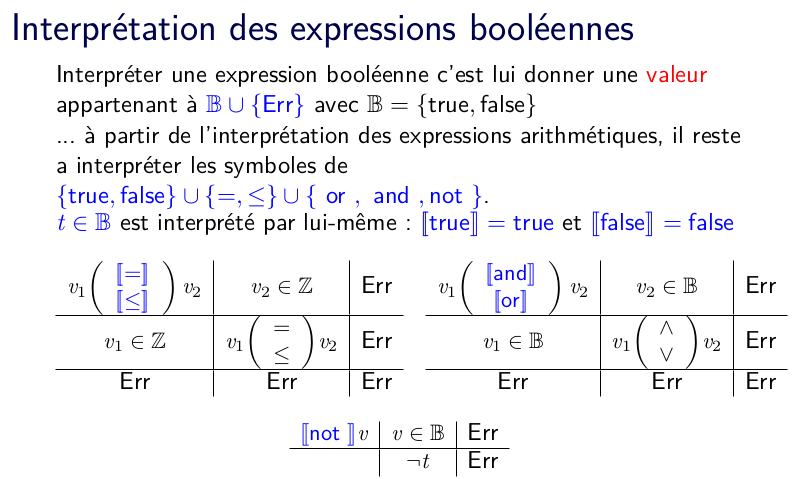
\includegraphics[height=4cm]{\Boolroot/interpretation.png}

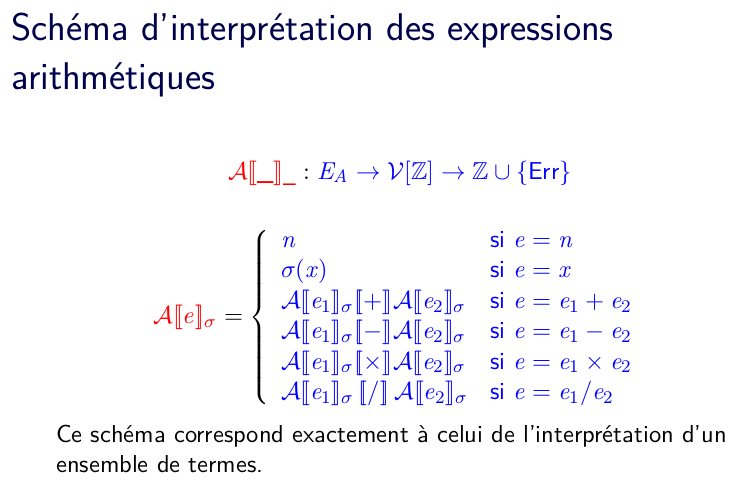
\includegraphics[height=4cm]{\Boolroot/schema_interpretation.png}

	\subsection{Traduction en OCaml}
	\lstinputlisting[language=OCaml, linerange={267-269,278-280,288-291,299-302,310-313}]{\OCamlroot/OCaml_exemple.ml}
	
	\lstinputlisting[language=OCaml, linerange={322-329}]{\OCamlroot/OCaml_exemple.ml}

	\subsection{Traduction en K}
	\lstinputlisting[language=K, linerange={53-84}]{\Kroot/K_exemple.k}


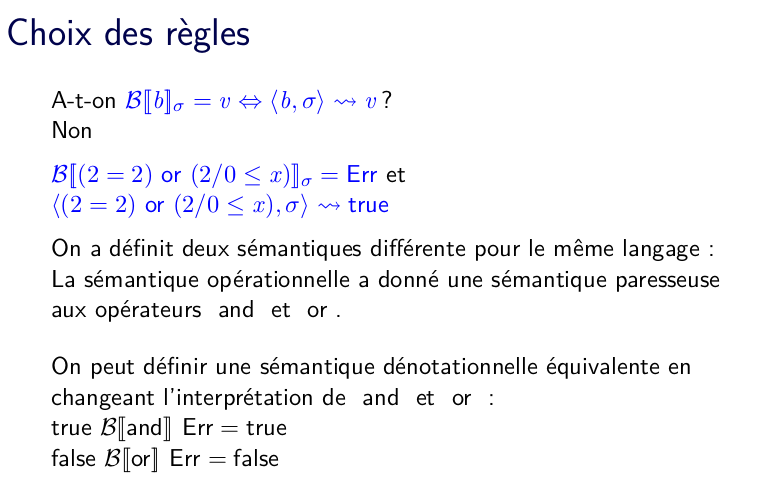
\includegraphics[height=4cm]{\Boolroot/choix_paresseux.png}










\section{Sémantique opérationnelle d’évaluation à grands pas}
Expressions booléennes équivalentes \\
$~$ est une congruence \\
Unicité d'un résultat

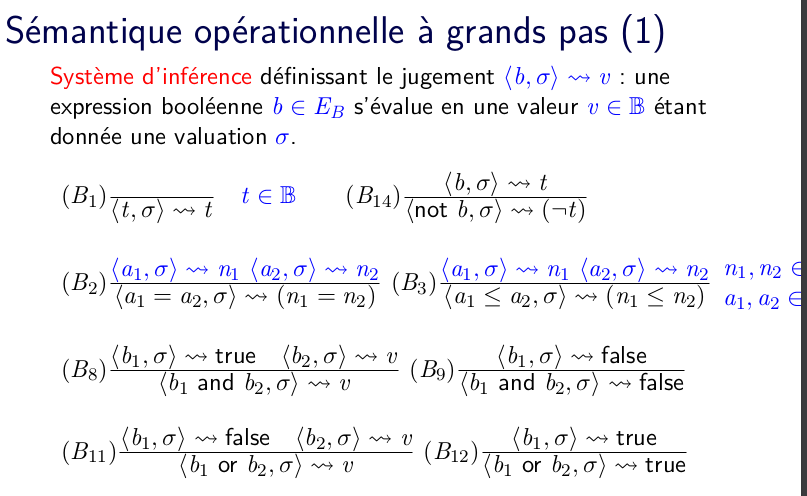
\includegraphics[height=4cm]{\Boolroot/eval_grands_pas.png}

\section{Sémantique opérationnelle d’évaluation à petits pas}
Exercice ?
	
	\subsection{Traduction en OCaml}

\lstinputlisting[language=OCaml, linerange={336-342}]{\OCamlroot/OCaml_exemple.ml}

\lstinputlisting[language=OCaml, linerange={353-362}]{\OCamlroot/OCaml_exemple.ml}

\lstinputlisting[language=OCaml, linerange={408-413}]{\OCamlroot/OCaml_exemple.ml}